% Fig. 4 -- Tier 1 passive banner-fingerprint drift, worked example (single column, 3.5 in).
% Compile with pdfLaTeX (Overleaf default). Output: fig04_tier1_drift.pdf
\documentclass[border=3pt]{standalone}
\usepackage[T1]{fontenc}
\usepackage{newtxtext,newtxmath}
\usepackage{tikz}
\usetikzlibrary{arrows.meta,positioning,calc}

\definecolor{acc}{RGB}{31,78,121}
\colorlet{accfill}{acc!10}

\tikzset{
  >={Stealth[length=3pt,width=2.6pt]},
  every node/.style={font=\footnotesize,inner sep=0pt},
  c0/.style={anchor=west},
  c1/.style={anchor=west},
  c2/.style={anchor=west},
  c3/.style={anchor=east},
  c4/.style={anchor=east},
  chg/.style={text=acc},          % changed field value
  rule/.style={line width=0.5pt,black},
}

\begin{document}
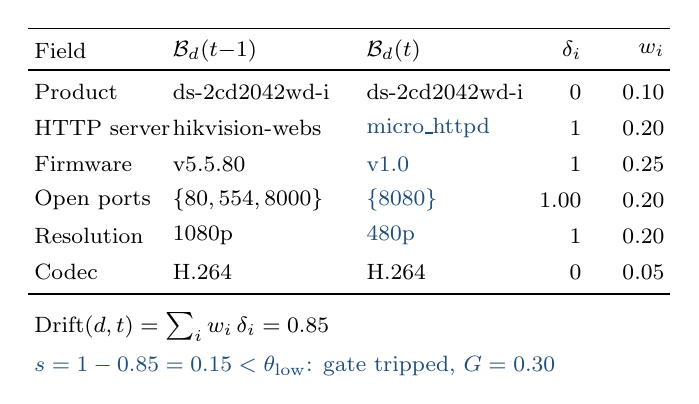
\begin{tikzpicture}[x=1pt,y=1pt]
  % column anchors: field 0, baseline 50, current 120, delta (right edge) 198, weight (right edge) 228
  \draw[rule] (-2,8) -- (230,8);
  \node[c0] at (0,0)   {Field};
  \node[c1] at (50,0)  {$\mathcal{B}_d(t{-}1)$};
  \node[c2] at (120,0) {$\mathcal{B}_d(t)$};
  \node[c3] at (198,0) {$\delta_i$};
  \node[c4] at (228,0) {$w_i$};
  \draw[rule] (-2,-7) -- (230,-7);

  % rows (pitch 13 pt)
  \node[c0] at (0,-15)  {Product};
  \node[c1] at (50,-15) {ds-2cd2042wd-i};
  \node[c2] at (120,-15){ds-2cd2042wd-i};
  \node[c3] at (198,-15){$0$};
  \node[c4] at (228,-15){$0.10$};

  \node[c0] at (0,-28)  {HTTP server};
  \node[c1] at (50,-28) {hikvision-webs};
  \node[c2,chg] at (120,-28){micro\_httpd};
  \node[c3] at (198,-28){$1$};
  \node[c4] at (228,-28){$0.20$};

  \node[c0] at (0,-41)  {Firmware};
  \node[c1] at (50,-41) {v5.5.80};
  \node[c2,chg] at (120,-41){v1.0};
  \node[c3] at (198,-41){$1$};
  \node[c4] at (228,-41){$0.25$};

  \node[c0] at (0,-54)  {Open ports};
  \node[c1] at (50,-54) {$\{80,554,8000\}$};
  \node[c2,chg] at (120,-54){$\{8080\}$};
  \node[c3] at (198,-54){$1.00$};
  \node[c4] at (228,-54){$0.20$};

  \node[c0] at (0,-67)  {Resolution};
  \node[c1] at (50,-67) {1080p};
  \node[c2,chg] at (120,-67){480p};
  \node[c3] at (198,-67){$1$};
  \node[c4] at (228,-67){$0.20$};

  \node[c0] at (0,-80)  {Codec};
  \node[c1] at (50,-80) {H.264};
  \node[c2] at (120,-80){H.264};
  \node[c3] at (198,-80){$0$};
  \node[c4] at (228,-80){$0.05$};

  \draw[rule] (-2,-88) -- (230,-88);

  % result
  \node[anchor=west] at (0,-100) {$\mathrm{Drift}(d,t)=\sum_i w_i\,\delta_i = 0.85$};
  \node[anchor=west,text=acc] at (0,-114) {$s = 1-0.85 = 0.15 < \theta_{\mathrm{low}}$: gate tripped, $G=0.30$};
\end{tikzpicture}
\end{document}
